
% Chapter 2

\chapter{Nuclear Matter: Hot and Cold} % Main chapter title
%----------------------------------------------------------------------------------------
\section{Hot Versus Cold Nuclear Matter}
Since the deconfinement of quarks corresponds to a condition where the temperature of the system is above some critical value, it is often called ``Hot Nuclear Matter.'' Therefore, the region of the nuclear matter phase diagram where quarks and gluons are confined or ``frozen'' into hadronic states is often called ``Cold Nuclear Matter.'' Historically, ``Hot'' QGP systems were created by colliding two large nuclei, such as in Au+Au collisions. In contrast,  ``Cold Nuclear Matter'' systems were studied by colliding smaller nuclei with large ones, such as in d+Au collisions, because it was believed that a large number of interacting quarks was needed in order to describe a thermal system undergoing a phase transition, and that small systems of few interacting quarks had an insufficient number of particles needed to describe such a system.

\section{The Cronin Effect}
The seminal paper titled \textit{Production of hadrons at large transverse momentum at 200, 300, and 400 GeV} by J.W. Cronin, et al. detailed a fixed target experiment that collided protons with a tungsten target and observed a phenomenon which typified cold nuclear matter systems. Later dubbed the \textit{Cronin Effect} after the paper's first author, the experiment found that the production of protons at mid $p_{T}$\footnote{Transverse momentum. Scalar quantity of momentum that is perpendicular to beam axis.} ($2\leq p_{T} \leq 4$) was enhanced when compared to the production of pions \citep{croninpaper}. Figure \ref{fig:croninratio} shows the production ratio of protons to pions over a range of transverse momentum. In order to measure how nuclear matter affects particle production compared to small systems, they defined a quantity called the \textit{number of effective nucleons}:
\begin{equation}
A_{eff} = \frac{\sigma_{absorption}}{\sigma_{pp}}, \qquad A^W_{eff} = \frac{1635\: mb}{40\: mb} = 40.9,
\end{equation}
where $\sigma_{absorption}$ is the absorption cross section of the target nuclei, $\sigma_{pp}$ is the total p+p cross section, and $A^W_{eff}$ is the number of effective nucleons with a tungsten target. In practice, the number of effective nucleons described the number of nucleons that interacted in the collision, with the limiting case of A=1 meaning p+p like collisions. The closed circle markers in Figure \ref{fig:croninratio} show the data from 23.7 GeV proton collisions on a fixed tungsten target; the open circles show the same data extrapolated to the lower limit of p+p like collisions.
\begin{figure}[H]
  \centering    
    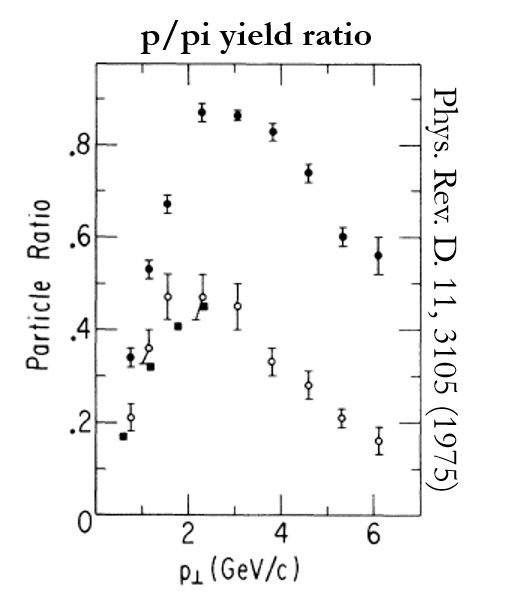
\includegraphics[width=0.5\textwidth]{prevplots/croninratio.JPG}
\rule{35em}{0.5pt}
  \caption[Proton vs pion yield ratio from the Cronin paper]{Proton vs pion yield ratio from the Cronin paper. Closed circles are the ratio obtained by colliding 23.7 GeV protons on tungsten ($A_{eff}= 40.9$). Open circles are the same data scaled to the low limit of single nucleon-nucleon interaction ($A=1$).}
  \label{fig:croninratio}    
\end{figure}

After the observation of this baryon enhancement in mid-$p_T$, many set out to come up with theoretical mechanisms that could explain this baryon production preference. The focus of these models was to describe the effect of the nuclear medium on incoming partons\footnote{The point-like objects that comprise hadrons described in a model proposed by Richard Feynman to analyze high energy collisions. We now know these \textit{partons} are quarks and gluons but the simplicity of the model lends itself well to describing these collisions and the terminology is still used today.}. Specifically, the models differentiated between \textit{soft, elastic} interactions and \textit{hard, inelastic} collisions of partons inside nucleons, and whether soft interactions happened before or after hard collisions. These mechanisms can then largely be categorized into two types, as follows: those where the incoming partons interact with the nuclear medium and those where outgoing partons, created after an incoming nucleon hard scatters, interact with the nuclear medium. These two categories are called \textit{Initial State Interactions} and \textit{Final State Interactions,} respectively.

\subsection{Initial State Multiple Scattering}
The first attempts at explaining the Cronin Effect were made using initial state interactions. K\"{u}hn, in 1975, described a mechanism where incoming partons scatter on nuclear partons, randomizing the direction of the incoming parton, before finally colliding with a nuclear quark to produce an event similar to a proton+proton collision \citep{PhysRevD.13.2948} (see Figure. \ref{fig:ISIscattering}). Since it is unclear how many ``soft scatters'' happen before the final hard scatter, the $p_{T}$ spectrum is broadened, which could account for the increase of particle production for the mid $p_{T}$ range. Furthermore, multiple soft scatters are unlikely to produce pions due to the high $p_T$ required to break color confinement, possibly explaining the mid $p_T$ baryon preference.
\begin{figure}[htbp!]
  \centering    
    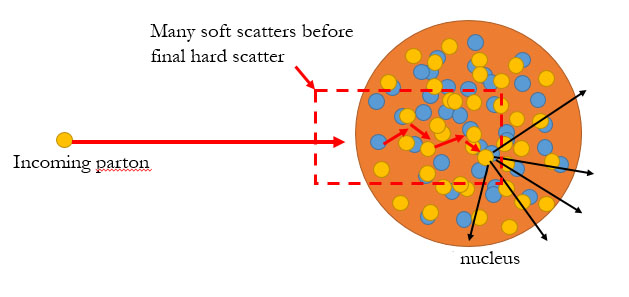
\includegraphics[width=0.8\textwidth]{Figures/ISIscattering.jpg}
\rule{35em}{0.5pt}
  \caption[Illustration of Initial State Multiple Scattering]{Illustration of Initial State Multiple Scattering.}
  \label{fig:ISIscattering}  
\end{figure} 

The NA10 collaboration at CERN set out to use back to back lepton probes to study the effect of the nucleus on outgoing parton showers created by hard scattering called \textit{jets}. They collided 140 GeV and 258 GeV negative pions on tungsten targets of various thicknesses and looked for muon pairs produced by quark-antiquark annihilation, also known as a \textit{Drell-Yan Process}.
%\begin{figure}[htbp!]
 % \centering
  %  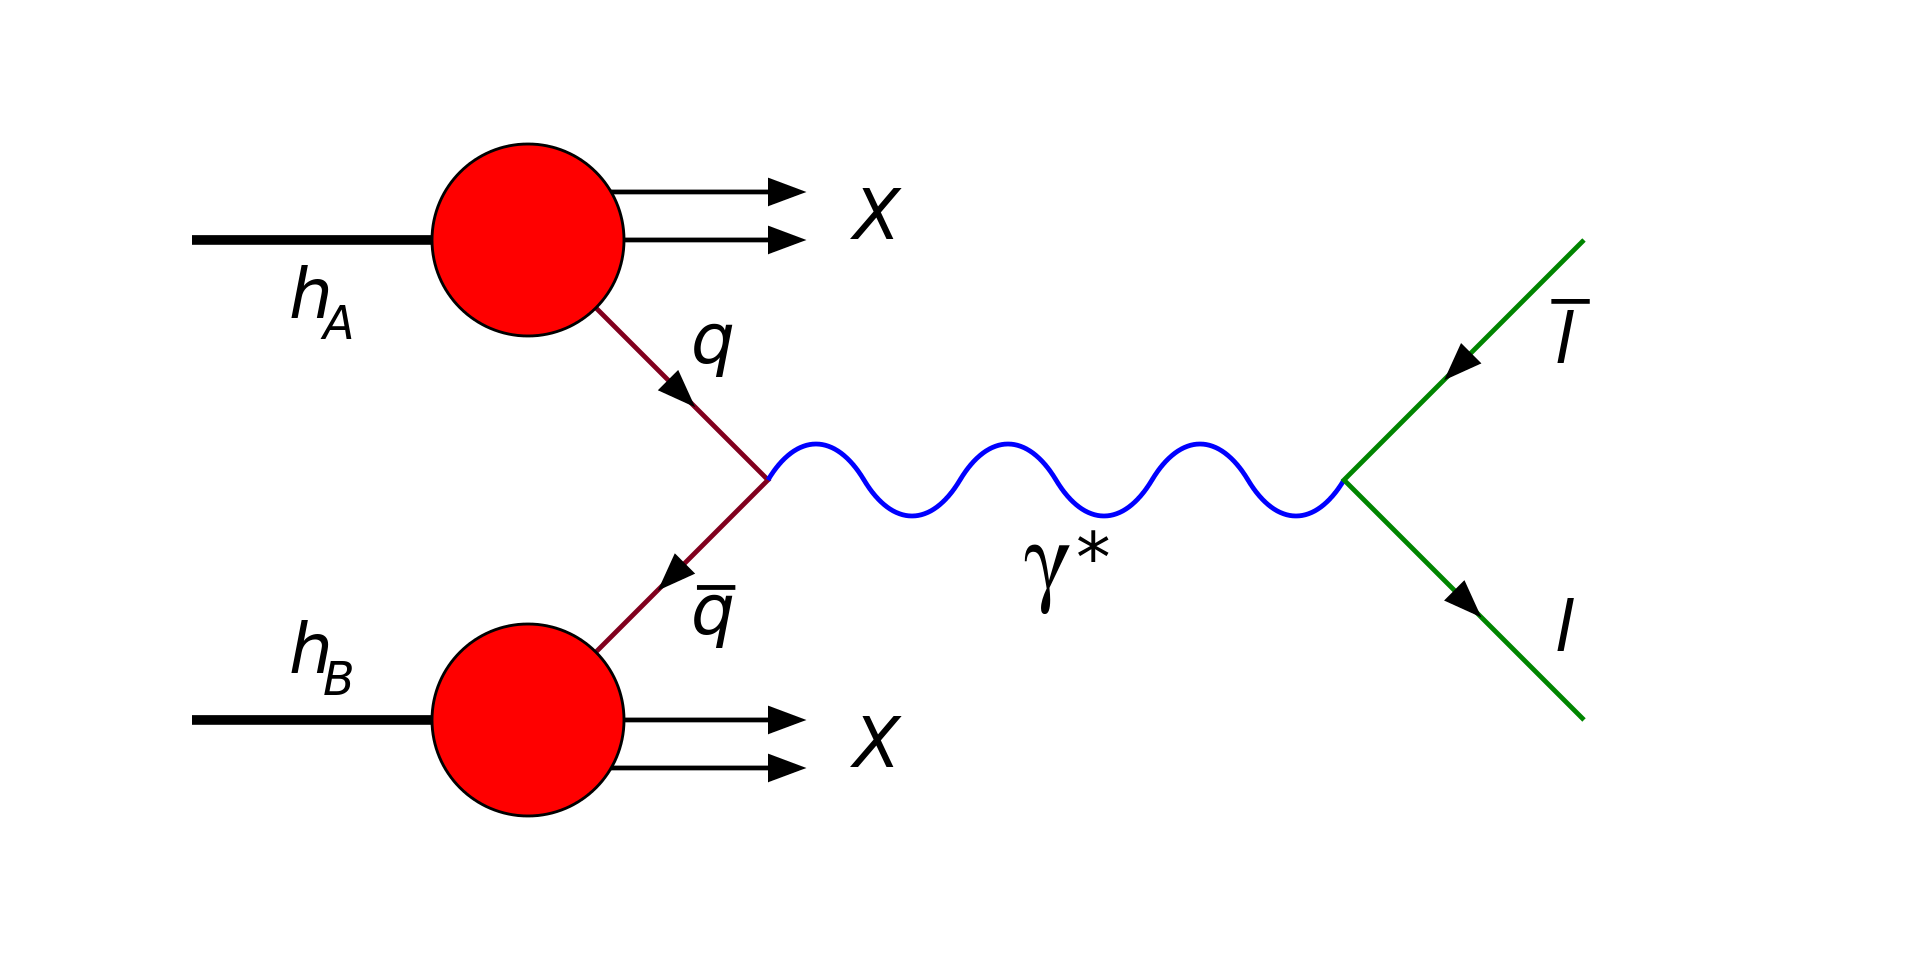
\includegraphics[width=0.7\textwidth]{Figures/DYfeynman.png}
  %  \rule{35em}{0.5pt}
  %\caption[Feynman diagram of Drell-Yan production of dileptons.]{Feynman diagram of Drell-Yan production of dileptons. Quark-Antiquark annihilation produces a lepton-antilepton pair through the exchange of a virtual photon.\citep{PhysRevLett.25.316}}
  %\label{fig:DYfeynman}
%\end{figure}
They found the mean squared $p_{T}$ of the muon pair did not vary substantially as a function of target thickness, which implies that incident partons are not affected by the thickness of the target and, therefore, the path length of soft scatters that would broaden the $p_{T}$ spectrum is very short. Furthermore, the E772 collaboration, with an experiment colliding 800 GeV protons on H$_{2}$, C, Ca, Fe, and W targets, showed that Drell-Yan produced dileptons’ mean squared $p_{T}$ did not vary much between the nuclear targets of varying nucleon number \citep{PhysRevLett.66.2285}, i.e., increasing the number of nucleons does not substantially change the net $p_{T}$, further showing that initial state contributions to $p_{T}$ broadening are minimal.

\subsection{Final State Multiple Scattering}
\begin{figure}[hbtp!]
\centering   
\begin{subfigure}[]{1\textwidth}\captionsetup{width=1.1\linewidth}
    \centering
    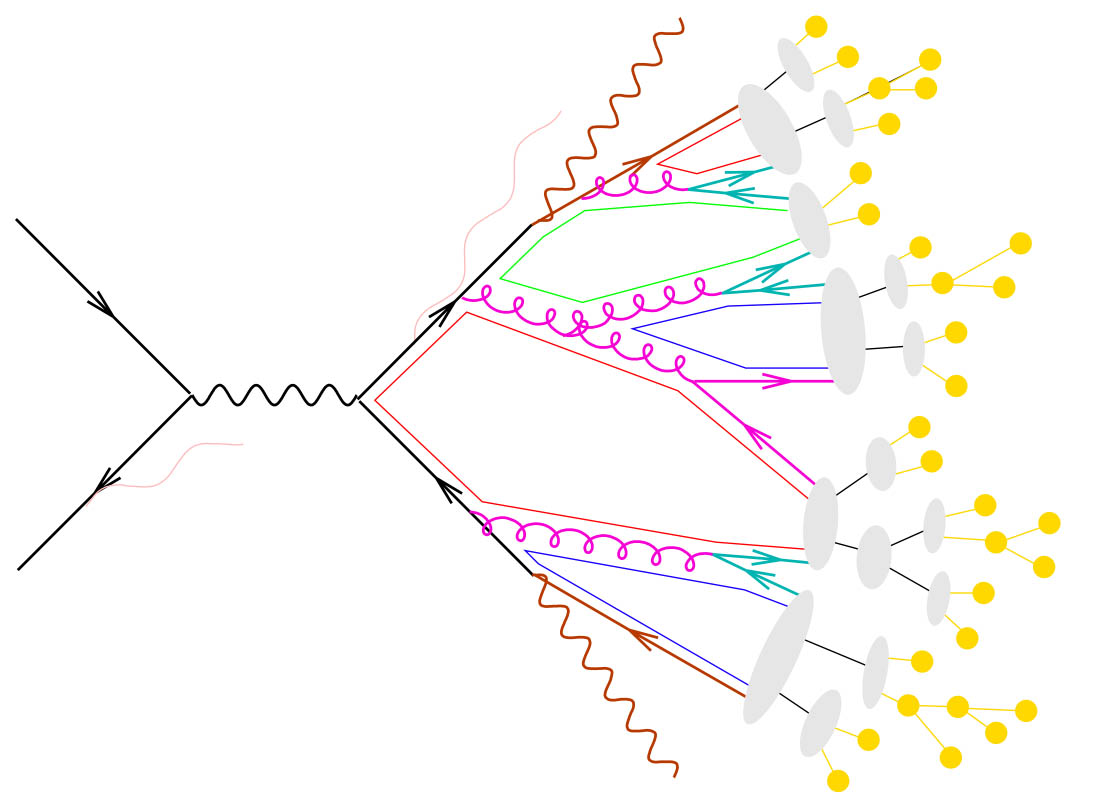
\includegraphics[width=0.5\textwidth]{Figures/jetfeynman.jpg}
\caption{A Feynman diagram \citep{jetfeynmancredit} depicting the annihilation of two quarks creating a force carrying boson which creates a quark-antiquark pair. By the rules of QCD confinement, single particles that have a color charge cannot exist by themselves. As they travel away from the vertex where they were formed they create other colored objects around them in a manner that the net color charge of all particles in the group is colorless. Each group of colorless particles is called a \textit{jet}. Since one jet forming quark is created going one direction, often another is formed going the opposite direction in order to conserve quantum numbers and momentum. This other quark in turn goes on to form its own jet in the same manner. This pair of jets is often referred to as a \textit{dijet}.}
\label{fig:jetfeynman}
\end{subfigure}
\begin{subfigure}[]{1\textwidth}
\captionsetup{width=1.5\linewidth}
    \centering
    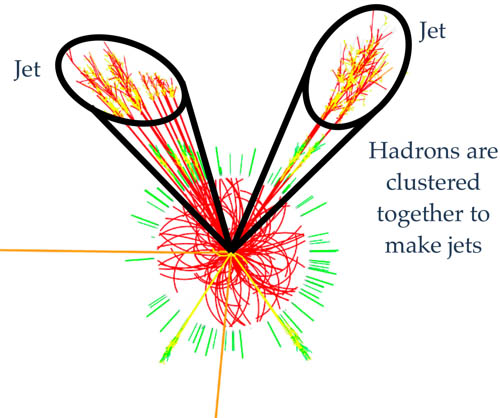
\includegraphics[width=0.5\textwidth]{Figures/jetdiagram.jpg}
\caption{A cartoon illustration \citep{jetdiagramcredit} of how this process might appear in an experiment.}
\label{fig:jetdiagram}
\end{subfigure} \rule{35em}{0.5pt}
\caption[Feynman and Cartoon diagrams of Jet Formation]{Two illustrations of how jets are formed in particle collisions.}
\label{fig:jetformation}    
\end{figure}
In 1991, the E609 collaboration at Fermilab studied phenomena in experiments that collided 400 GeV/c protons with hydrogen and lead targets \citep{Corcoran:1990vq}. The conditions of interest were the creation of two back-to-back jets (dijets) produced after an incoming parton hard scattered with a target nucleon\footnote{Figure \ref{fig:jetformation} describes the formation of dijets.}. Since the dijets are produced back to back, they start with the same momentum. Any difference between two jets' momentum could therefore be attributed to a final state interaction. They defined a quantity called \textit{planarity} which measured how back-to-back two jets are. In their words:
\begin{addmargin}[1.5em]{2em}
``An axis is found which maximizes the sum of the squares of all momentum components ($b_{max}$) along that axis while minimizing the sum of the squares of momentum components perpendicular to that axis ($b_{min}$). Planarity is then defined as: 
\begin{equation}
P = \frac{b_{max}-b_{min}}{b_{max}+b_{min}}.
\end{equation}
For two narrow back-to-back jets, P approaches 1, while for a circularly symmetric event P is 0.''
\end{addmargin}

\begin{figure}[h]
  \centering
    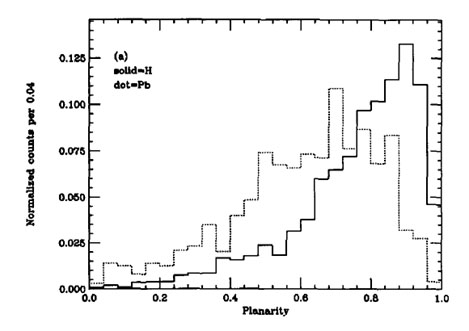
\includegraphics[width=0.75\textwidth]{prevplots/e609planarity.jpg}
    \rule{35em}{0.5pt}
  \caption[Planarity of jets created with protons incident on Pb targets vs H targets.]{Planarity of jets created with protons incident on Pb targets vs H targets.  \citep{PhysRevLett.70.143}}
  \label{fig:e609planarity}
\end{figure}
The E609 measurement (Figure \ref{fig:e609planarity}) compared the planarity of dijets created from protons colliding with a hydrogen target with the planarity of those created with collisions on a lead target. They noticed a downward shift in planarity and broadening of the spectrum for Pb dijets compared to H although both had very similar jet widths. This measurement led to a paper in 1993 where they concluded that ``parton hard scatterings within nuclei involve very little nuclear scattering of the incident parton, but that there is substantial nuclear rescattering of outgoing hard scattered partons.'' \citep{PhysRevLett.70.143} Because of this, we call this type of mechanism a \textit{Final State Interaction} (for example, see Figure \ref{fig:FSIscattering}). While it is true that this could account for the increase in particle production, it does not effectively explain why the effect is stronger for baryons than for mesons and why this preference disappears for at high $p_{T}$.
\begin{figure}[htbp!]
  \centering
    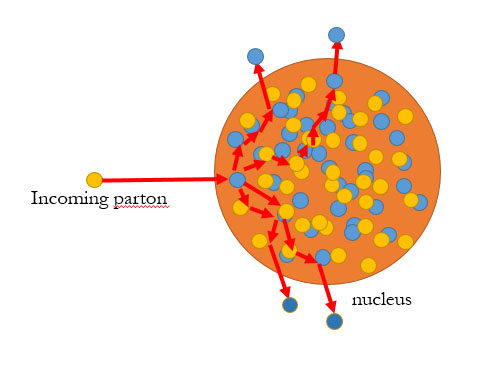
\includegraphics[width=0.7\textwidth]{Figures/FSIscattering.jpg}
   \rule{35em}{0.5pt}
  \caption[Illustration of Final State Multiple Scattering]{Illustration of Final State Multiple Scattering.}
  \label{fig:FSIscattering}
 \end{figure} 

\section{Hot Nuclear Matter: Quark Gluon Plasma }
So far, this discussion has remained within the hadronic temperature regime\footnote{That is, where quarks and gluons are confined to hadronic states.}. As summarized in the previous chapter, physicists had already seen hints that new physics was taking place when the energy density reached some critical value, and consequently RHIC was commissioned to study this phase change.

\subsection{Collective Flow}
As mentioned, one of the signatures of this phase change was that the medium behaved collectively and that, like a fluid, it flowed. \textit{Collective flow} of the medium could be measured by the varying distribution of particles produced about the azimuth, or the \textit{azimuthal anisotropy}. This anisotropy is a measure of how a pressure anisotropy caused by the initial conditions of an ion-ion collision can be correlated to a momentum anisotropy of outgoing particles about the azimuth of the collision. The details of this pressure anisotropy scale with a parameter called collision \textit{centrality}, which is discussed in detail in Section \ref{sect:centrality}, but for simplicity we can think of centrality as how ``head-on'' the collision of two ions is, i.e., if they collide with a large overlap or a small one. A large overlap creates a circular shaped pressure gradient whereas a small overlap creates an elliptic shaped pressure gradient as shown in Figure \ref{fig:centvsperiph1}.

\begin{figure}[htbp]
\centering
    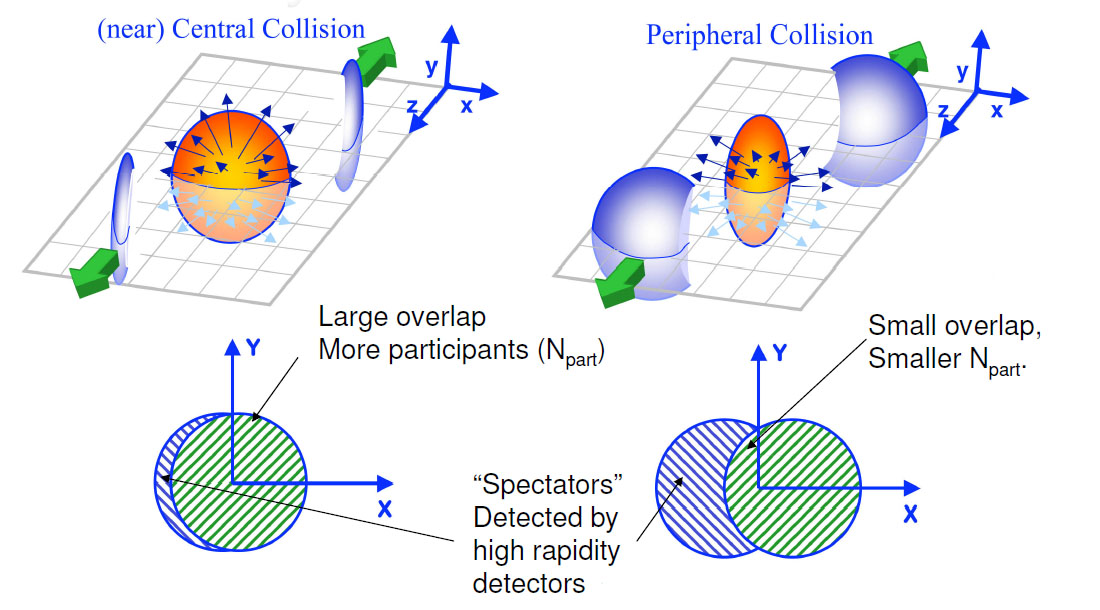
\includegraphics[width=1\textwidth]{Figures/centralvsperipheral.jpg}    
\rule{35em}{0.5pt}
	\caption[Central vs Peripheral collisions, geometry of initial conditions]{An illustration of central vs peripheral heavy ion collisions, geometry of initial conditions. The beam axis goes into and out of the page for the lower diagrams.}
\label{fig:centvsperiph1}
\end{figure}

It follows, then, that mid-peripheral collisions create the largest azimuthal pressure anisotropy, and therefore would result in the largest momentum anisotropy of outgoing particles. This pressure anisotropy is largest around the waist of the collision region and weakest at the poles, meaning that the collective flow of the QGP would happen with an elliptical shape, also called \textit{elliptic flow} (see Figure \ref{fig:v2auau}), measured by the quantity $v_2$\footnote{There are other types of flow which will be discussed further in Chapter \ref{sect:flow}.}.
    
\begin{figure}[htbp]
\centering 	
    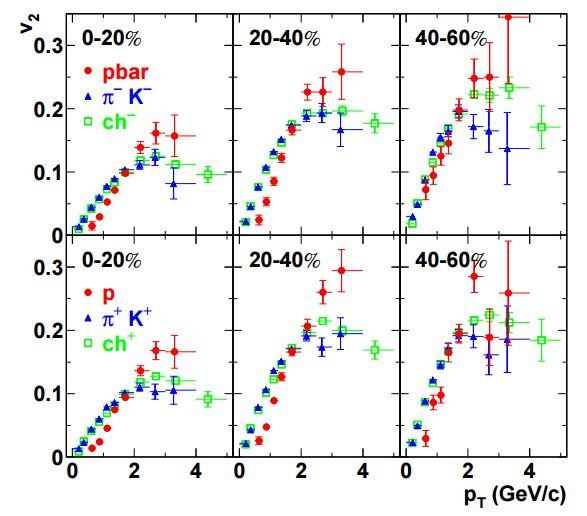
\includegraphics[width=0.5\textwidth]{prevplots/v2auau.jpg}
\rule{35em}{0.5pt}
	\caption[Identified particle elliptic flow vs centrality in 200 GeV Au+Au collisions]{Identified particle elliptic flow vs centrality in 200 GeV Au+Au collisions. Flow is strongest for peripheral collisions due to initial pressure anisotropy indicative of QGP collective behavior. \citep{Adler:2003kt}}
\label{fig:v2auau}	
\end{figure}

\subsection{Baryon Enhancement}

\begin{figure}
\centering    
\begin{subfigure}[b]{0.8\textwidth}
    \centering
    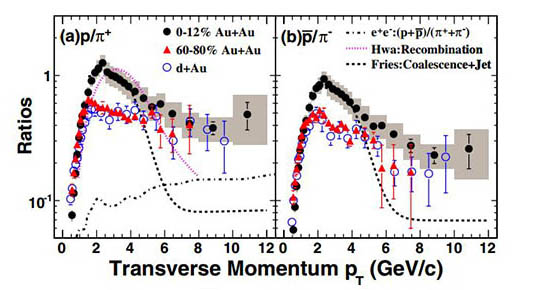
\includegraphics[width=\textwidth]{prevplots/ppiratiocentvsperiph.JPG}
    \caption{ $p/\pi{+}$ and $\bar{p}/\pi^{-}$ ratios for central and peripheral 200 GeV Au+Au collisions. Two leading models are compared to the data as well as the same ratio for 200 GeV d+Au collisions. \citep{PhysRevLett.97.152301}}
    \label{fig:ppiratiocentvsperiph}
\end{subfigure}
\rule{35em}{0.5pt}
\begin{subfigure}[b]{0.9\textwidth}
    \centering
    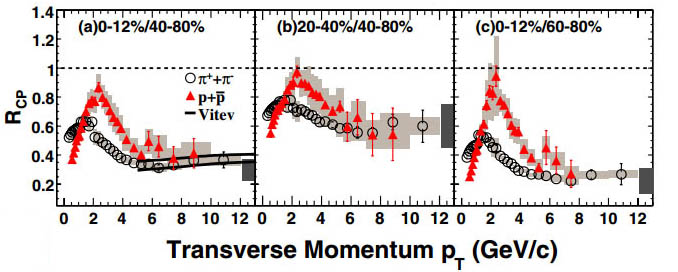
\includegraphics[width=\textwidth]{prevplots/Rcpcentvsperiph.jpg}
    \caption{Nuclear modification factor, $R_{CP}$, comparing nuclear effects on particle production in central versus peripheral Au+Au collisions compared to production in binary scaled p+p collisions (see appendix \ref{nuclmodfactapp} for a summary on nuclear modification factors). \citep{PhysRevLett.97.152301}}
    \label{fig:Rcpcentvsperiph}
\end{subfigure}
\rule{35em}{0.5pt}
\caption[Evidence of Baryon Enhancement in Au+Au collisions]{$p/\pi$ production ratio and $R_{CP}$ as evidence of Baryon Enhancement in central Au+Au.}
\label{fig:baryonenhancementAA}    
\end{figure}

Another surprising feature of this new phase of matter was the way particles were created from the QGP, namely how it differed from simpler p+p collisions. Particle production in p+p collisions is statistically well-understood for common particles such as pions and protons, and so the particle yields of these were compared to the particle yields of the same in heavy ion systems. If ion collisions behaved no differently than p+p collisions, then one would expect these yields to simply scale by some value proportional to the number of nucleon-nucleon collisions. That is, if two ions each containing N nucleons collided, then we would expect the yields to increase by a factor proportional to N, since a system of N colliding nucleons describes the number of p+p-like collisions. An indication that heavy ion systems were different was that the particle yields were different from those expected from scaling p+p collisions, specifically that particles containing three quarks (baryons) were produced in greater abundance compared to those containing two quarks (mesons) in peripheral Au+Au collisions \citep{PhysRevLett.97.152301}. This result is shown in Figure \ref{fig:ppiratiocentvsperiph} and shows the comparative yield between protons and pions in bins of $p_{T}$. The phenomenon of interest is the apparent baryon excess, or \textit{baryon enhancement}, in the central collision data set for the mid $p_{T}$ range, which is strongest at around $p_{T}\approx$ 2 GeV/c and disappears at around $p_{T}\approx$ 4 GeV/c. Similarly, the \textit{Nuclear Modification Factor}\footnote{See Appendix \ref{nuclmodfactapp}.} for central and peripheral collisions also shows this enhancement in the same range (shown in Figure \ref{fig:Rcpcentvsperiph}). Though this enhancement is similar to the Cronin effect in cold systems, the Cronin effect had already been attributed to multiple scattering effects of partons on ``frozen'' hadronic states, whereas the asymptotic freedom of quarks in the QGP would not cause the same scattering effects since the whole system was outwardly expanding.

\subsection{Theoretical Models of the QGP Hadron Interaction}
Though many have proposed models to describe this baryon enhancement, this discussion will focus on a handful of leading models. They each describe the following various parts of the collision evolution: the description of the nuclei before collision, the moments directly after a collision when the system equilibrates, the behavior of the equilibrated phase, and the freeze-out mechanism.

\subsubsection{Relativistic Hydrodynamics}
Luzum and Romatschke \citep{PhysRevC.78.034915} proposed treating the collective flow of the equilibrated QGP as a \textit{hydrodynamic} problem. That is, they sought to treat the QGP as a \textit{relativistic viscous fluid} since it flowed like a fluid composed of strongly interacting particles traveling at relativistic speeds. Following the relativistic energy-momentum equations for a fluid with shear viscosity, they found that the strength of QGP elliptic flow depended on the ratio of the medium's shear viscosity and the entropy density. Furthermore, they made an important distinction between the rapidly evolving period just after the collision and the time described by the collective behavior of an equilibrated phase. The process of equilibration between the moment of collision and the equilibrated QGP is called \textit{thermalization} and describes the conversion of relativistic ion kinetic energy before collision into deconfined quark matter thermal energy after collision. Their distinction was that this thermalization phase was not required to be very small\footnote{$\tau_0 < 1$ fm/c ($\sim 3 \times 10^{-24}$ sec), a.k.a. ``early thermalization''.}, and that many details could be garnered from the duration and mechanism of this thermalization process such as the eccentricity of the elliptic flow. Since the QGP consists of deconfined quarks, the hydrodynamic model suggests that baryon excess in flow could be attributed to the number of constituent quarks in the hadron. That is, mesons and baryons should flow the same if scaled by the number of quarks they contain\footnote{Two quarks for mesons, three quarks for baryons.}, a property that experiments at RHIC\footnote{PHENIX and STAR} have observed and that is shown in Figure \ref{fig:quarkscaledv2}.

\begin{figure}[H]
  \centering   
    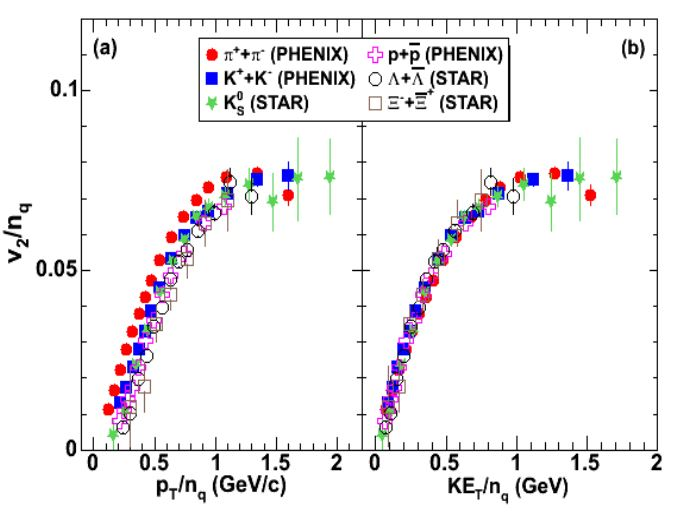
\includegraphics[width=0.7\textwidth]{prevplots/quarkscaledv2.JPG}
  \rule{35em}{0.5pt}
  \caption[Quark Scaled Elliptic Flow Results from PHENIX and STAR in Au+Au $\sqrt{s_NN}=200 GeV$ collisions]{Quark Scaled Elliptic Flow Results from PHENIX and STAR \citep{velkovska:lec12} in Au+Au $\sqrt{s_{NN}}=200 GeV$ collisions. Left plot shows flow vs (quark scaled) transverse momentum, right plot tests for partonic degrees of freedom by plotting vs transverse kinetic energy.}
  \label{fig:quarkscaledv2}  
\end{figure} 

\subsubsection{Recombination and Fragmentation}
Following the idea that a phase change in nuclear matter happens when a critical energy density deconfines quarks and gluons from their bound states as neutrons and protons, and that the post-collision evolutionary behavior of this QGP is one that expands rapidly, Rudolph Hwa and C.B. Yang postulated that the enhancement of particle production could be explained with a freeze-out mechanism, namely by the ways in which the outgoing partons interacted \citep{PhysRevC.70.024905}. They defined two momentum classifications for outgoing partons: \textit{soft} partons with low transverse momentum (in the hundreds of MeV/c) created by the collective thermal expansion of the QGP, and \textit{hard} partons with high transverse momentum created by hard nuclear scattering processes. Since these hard partons result in jet formation, and jets are comprised of a shower of particles, they use the terminology \textit{shower parton} to describe these hard scatter produced partons. The production of particles could then be described by the way these various partons combined to produce hadrons, i.e., the way soft partons combined with other soft partons, the way they combined with hard partons, and the way hard partons combined with other hard partons. This mechanism was termed \textit{recombination} since it relied on the recombining of quarks in partons created from the nuclear collision.

\begin{figure}
\centering    \rule{35em}{0.5pt}
\begin{subfigure}[b]{0.32\textwidth}
    \centering
    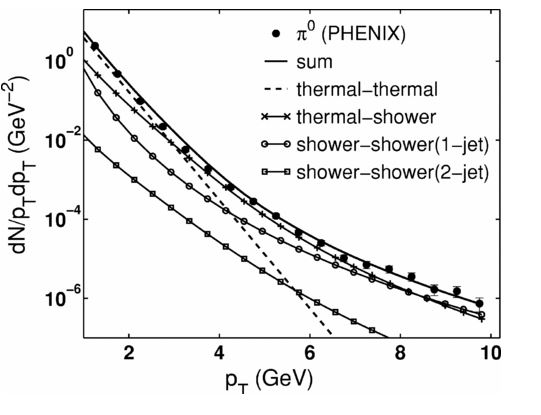
\includegraphics[width=\textwidth]{prevplots/piyieldrecomb.JPG}
    \caption{$p_T$ distribution of pions}
    \label{fig:kyieldrecomb}
\end{subfigure}
\begin{subfigure}[b]{0.32\textwidth}
    \centering
    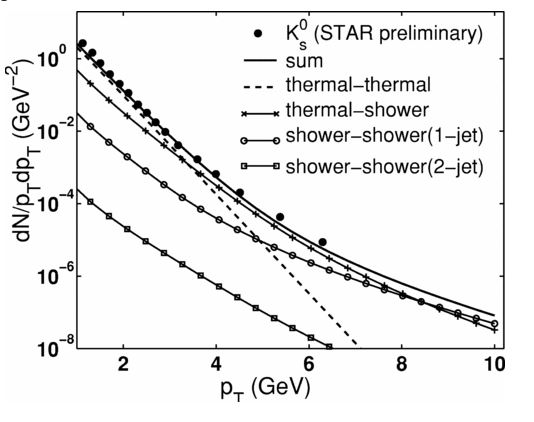
\includegraphics[width=\textwidth]{prevplots/kyieldrecomb.JPG}
    \caption{$p_T$ distribution of kaons}
    \label{fig:kyieldrecomb}
\end{subfigure}
\begin{subfigure}[b]{0.32\textwidth}
    \centering
    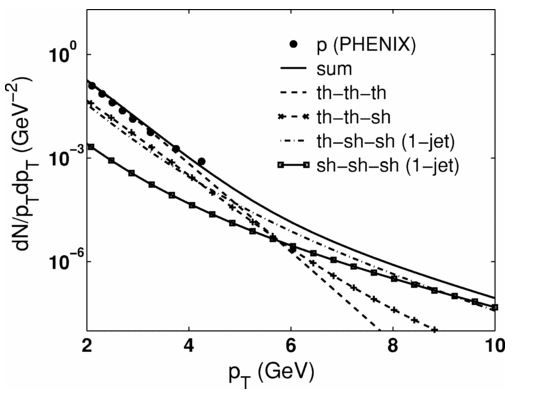
\includegraphics[width=\textwidth]{prevplots/pyieldrecomb.JPG}
    \caption{$p_T$ distribution of protons}
    \label{fig:pyieldrecomb}
\end{subfigure}
\begin{subfigure}[b]{0.5\textwidth}
    \centering
    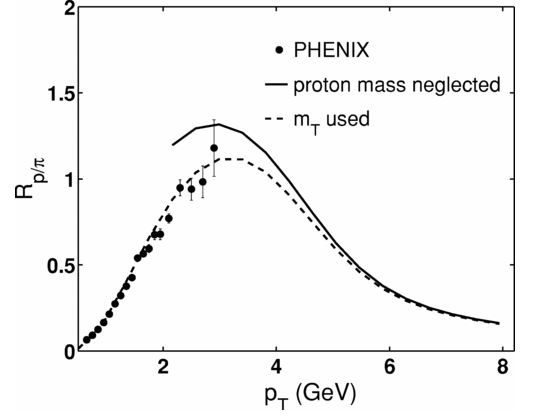
\includegraphics[width=\textwidth]{prevplots/ppiratiorecomb.JPG}
    \caption{$p/\pi$ production ratio versus $p_T$}
    \label{fig:ppiratiorecomb}
\end{subfigure}
\rule{35em}{0.5pt}
\caption[Recombination model compared with Au+Au data]{Au+Au identified particle measurements compared with recombination model predictions. For the $p_T$ distributions we see three distinct regions of recombination, the low $p_T$ range where soft thermal parton recombination dominates, the high $p_T$ range where hard parton recombination dominates, and the middle range where thermal-hard recombination best describes the data. \citep{PhysRevC.70.024905}}
\label{fig:hwaAAmodels}    
\end{figure}

\begin{figure}[htbp!]
  \centering  
    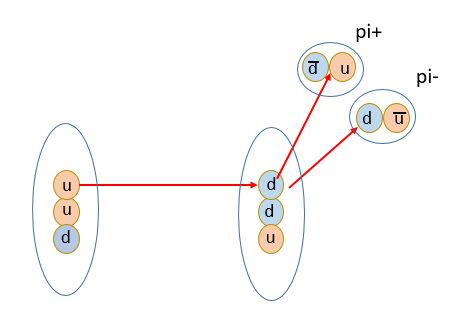
\includegraphics[width=0.5\textwidth]{Figures/fragmentationdiag.JPG}
 \rule{35em}{0.5pt}
  \caption[Illustration of an example hard scatter resulting in fragmentation to two pions]{Illustration of an example hard scatter resulting in fragmentation to two pions. Here an up quark scatters with enough energy to scatter and release the down quark from being bound in another nucleon. This occurs with enough energy to create antiparticle partners from the vacuum resulting in the formation of charged pions.}
  \label{fig:fragmentationdiag}   
\end{figure} 
Fries, M{\"u}eller, et al. simplified this picture, postulating that the reason protons were produced in abundance was simply that, following a collision, the quark building blocks of protons\footnote{That is, up and down quarks.} are plentiful and that they simply recombine back into their confined states. This mechanism dominates for low $p_{T}$ (soft partons) since outgoing partons are traveling slowly enough that the constituent quarks remain connected due to color confinement. In contrast, hard partons are more likely to have enough energy to briefly break color confinement, thereby isolating quarks into \textit{fragments} which then create jets of quark/anti-quark pairs, i.e., mesons. This two-regime model naturally creates a baryon preference for low $p_{T}$ partons by recombination that is met with proportional meson production when the parton $p_{T}$ is adequately high enough for fragmentation (see Figure \ref{fig:hwaAAmodels}).


\section{Collective Flow at the LHC}
Until now, it had appeared as if the lines in the proverbial sand were clear with respect to the nuclear matter phases and that we had two distinct ways with which to describe the properties of these two states. On the one side, there was cold, hadronic\footnote{Quarks confined in hadron states.} matter which had its own experimental signatures that could be observed in the collisions of light ions with heavy ones (such as d+Au). On the other hand, there was hot, deconfined, quark matter which behaved another way and was measured using collisions of two heavy nuclei (as in Au+Au). This notion that the two experimental methods allowed the temperature dependent phenomena to be studied separately was brought into question in 2015 when the \textit{Large Hadron Collider} (LHC) at CERN turned on and entered its second era of measurements. At the Compact Muon Solenoid (CMS) they collected data from p+p and p+Pb collisions at 5.02 TeV and compared it to Pb+Pb collisions at 2.76 TeV \citep{Khachatryan:2015waa}. While hydrodynamic phenomena like collective flow was expected in the Pb+Pb data, they did not expect to find flow in systems consisting of a small number of interacting nucleons such as p+Pb (see Figure \ref{fig:pPbflow}).
 
The appearance of flow in systems previously thought of as ``cold'' was a sign that perhaps the QGP forms much more easily than was previously expected and that perhaps some phenomena found in cold systems, such as baryon enhancement, could be attributed to mechanisms used to explain similar phenomena in hot heavy ion systems.

\begin{figure}[H]

    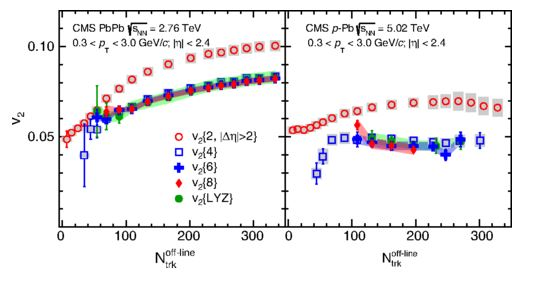
\includegraphics[width=1\textwidth]{prevplots/pPbflowLHC.JPG}
\rule{35em}{0.5pt}
  \caption[Elliptic Flow in p+Pb at the LHC]{CMS result from 5.02 TeV p+Pb collisions showing a nonzero elliptic flow signal versus track multiplicity. \citep{Khachatryan:2015waa}}\label{fig:pPbflow}
\end{figure} 

\section{Recombination and Fragmentation for All?}
\label{sect:recombcold}
Furthermore, experimental evidence that the two systems behave quite similarly has been found. In Figure \ref{fig:daaaratios} particle production ratios ($p/\pi$) are compared and it is seen that the baryon enhancement, which was indicative of the QGP formation in peripheral Au+Au collisions, is followed extremely closely by data from central d+Au. 

\begin{figure}[htbp!]
  \centering    
    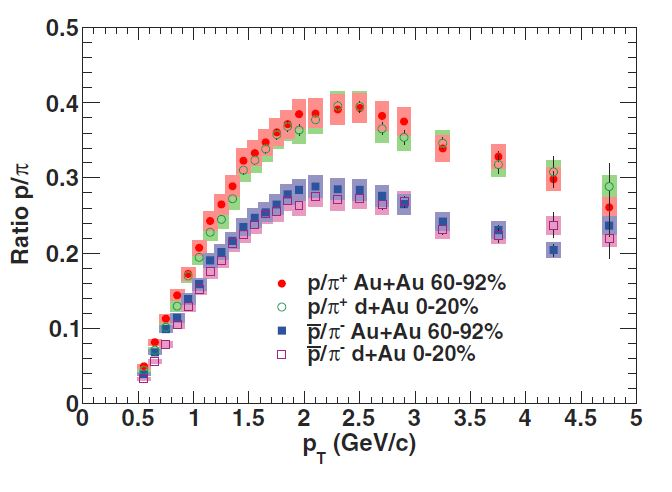
\includegraphics[width=0.7\textwidth]{prevplots/dAvsAAratios.JPG}
\rule{35em}{0.5pt}
  \caption[p/$\pi$ ratios compared for central d+Au and peripheral Au+Au]{p/$\pi$ ratios compared for central d+Au and peripheral Au+Au \citep{PhysRevC.88.024906}.}
  \label{fig:daaaratios}    
\end{figure} 

It may seem that the behaviors of the two results in Figure \ref{fig:daaaratios} are contradicting since the effect happens in central events for the d+Au system but in peripheral events in the Au+Au system, but it is seen upon inspection that the two cases are similar. In the Cronin result, the quantity of effective nucleons described the number of nucleons that interacted in a system. If we make the hypothesis that the QGP would most likely form with a higher number of interacting nucleons, then it follows that, if a QGP were to be formed in d+Au, it would be most likely to form in central collisions. And so, since physicists love reductionism and unification, and that the evidence makes one wonder if a QGP is formed in these simpler systems, it would be advantageous to be able to describe the two systems with a single mechanism.

Are there even the building blocks to support such a notion that QGP is created in such a simple system as d+Au? Recombination is easy to justify in Au+Au since the large number of interacting nucleons makes the formation of the QGP easily achieved and leaves a great abundance of free quarks that are able to recombine. Could there be analogous members at work in the d+Au system? 
%\begin{figure}[b!]
%  \centering
%    \rule{35em}{0.5pt}
%    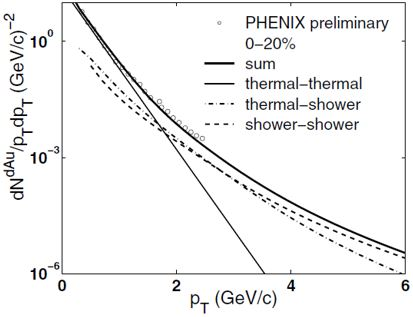
\includegraphics[width=0.5\textwidth]{prevplots/daurecomb.JPG}
%  \caption[Pion transverse momentum distribution from d+Au collisions compared to one created with the recombination model]{Pion transverse momentum distribution from d+Au collisions compared to one created with the recombination model}
%  \label{fig:daurecomb}
%    \rule{35em}{0.5pt}
%\end{figure}
Hwa and Yang set out to adapt their recombination model to fit the phenomena in d+Au \citep{PhysRevLett.93.082302}. They asserted that since hard scattering creates jets, jets traversing the nuclear medium generate many soft outgoing partons. They argue that these soft partons could behave like an expanding QGP, that is to say, they behave like the thermal partons in Au+Au collisions. Since thermal parton recombination seems to explain baryon enhancement well, and if soft partons behave like thermal partons, could there be recombination in d+Au as well? Additionally, if there is, could it be a sign that we should see other signs of QGP formation, such as collective flow? 

\section{The Big(ger) Picture}
What other phenomena could hint at the formation of a QGP? Many of the mechanisms discussed thus far pertain to the collective behavior post-thermalization, that is, the nature of the thermal-equilibrated quark fluid and its subsequent hadronization or \textit{freeze-out}. However, as noted when discussing the hydrodynamic model, the initial conditions of the relativistic ions and the intermediary evolution of the thermalization process had proven to affect the behavior of the created QGP. These are the leading models of the initial conditions that precede the equilibrated QGP state.

\begin{figure}[b!]
  \centering

    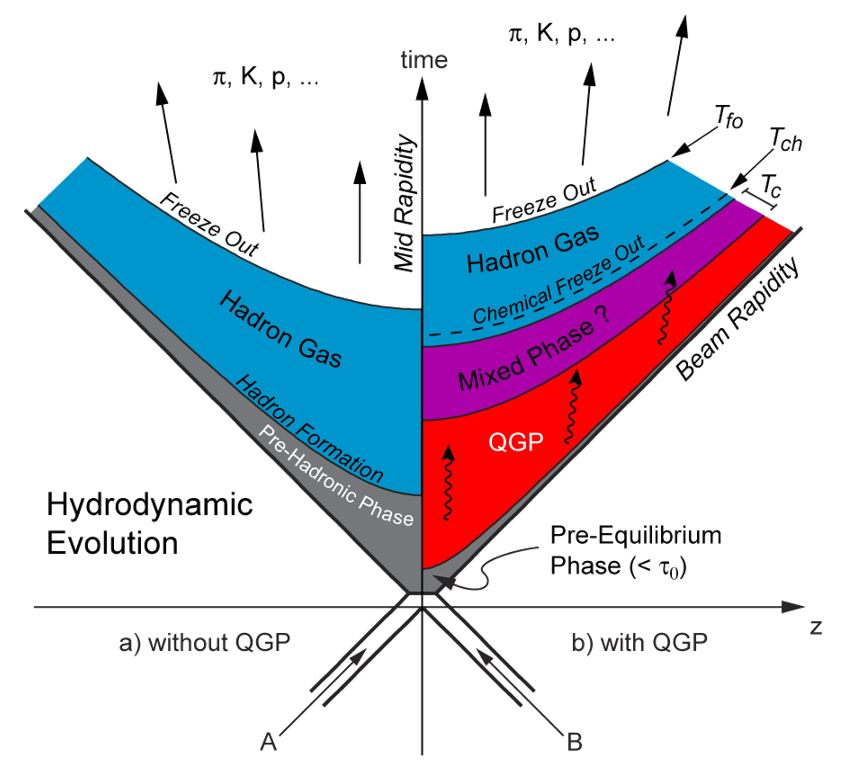
\includegraphics[width=0.5\textwidth]{Figures/hydrodynamicevolution.JPG}
\rule{35em}{0.5pt}
  \caption[A diagram of QGP hydrodynamic evolution.]{A diagram of QGP hydrodynamic evolution.}
  \label{fig:hydroevolution}

\end{figure}

\subsection{The Glauber Model}
\label{sect:glauber}
The Glauber Model of nuclear interaction, developed by Roy Glauber, pioneered the use of quantum mechanical scattering for systems comprised of many particles. It treats the nucleus as a distribution of nucleons over the volume of a sphere that can be reduced to a continuous nucleon density distribution as a function of the nucleus' radius \citep{Miller:2007ri}. Glauber pictured the collisions of two nuclei as a sequence of collisions involving the constituent nucleons within them. Specifically, that the number of these collisions could be counted by assuming inbound particles travel in straight lines through a nucleus. When combined with the cross sectional nucleon density distribution, it followed that the resulting number of interactions depended on the radius from the center of the nucleus with which the colliding nucleon's trajectory passed through, as shown in Figure \ref{fig:glaubermodel}.
\begin{figure}[b!]
  \centering

    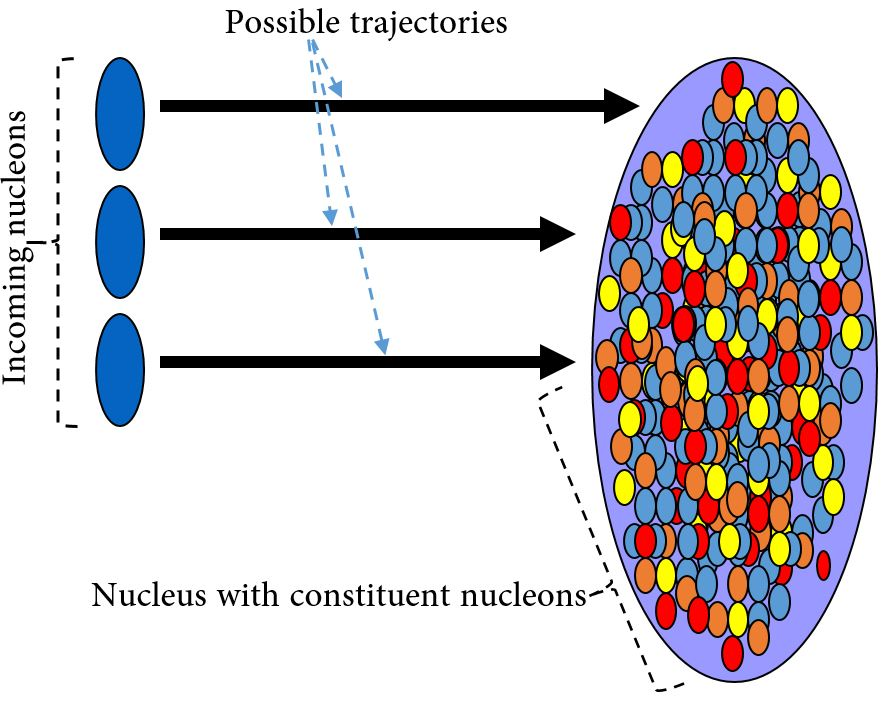
\includegraphics[width=0.5\textwidth]{Figures/glauberpic.jpg}
    \rule{35em}{0.5pt}
  \caption[A cartoon of the Glauber Model]{A Cartoon of the Glauber Model. The density of constituent nucleons varies by radius. Nucleons from incident nucleus interact with a variable number of nucleons in the other nucleus depending on the radius of the possible trajectory from the center of that nucleus. \citep{Nagle:2006}}
  \label{fig:glaubermodel}

\end{figure}

The Glauber model is easy to grasp from first principles and is useful for describing such quantities as the multiplicity of produced particles as a function of centrality. It relies very little, however, on the forces at work within the nucleus and physics of matter at relativistic speeds. We know that objects with relativistic velocities experience various effects such as length contraction and time dilation. Additionally, there has been much theoretical work on how the constituents of a nucleus change in the context of asymptotic freedom along with growing collision energy \citep{PhysRevD.10.1649}.

\subsection{Color-Glass Condensate}
A leading model that describes the behavior of nuclei at ultra-relativistic speeds is the \textit{Color-Glass Condensate} (CGC). The H1 and ZEUS experiments at the Hadron Electron Ring Accelerator (HERA) in Germany studied the structure of protons by colliding them with electrons at a center-of-mass energy of 318 GeV \citep{Abramowicz2015}. Their experiments better mapped the \textit{Parton Distribution Function} (PDF), which describes the probability density of particles versus fractional longitudinal momentum. This momentum, the Bjorken \textit{x} ($x_{B}$), is how much of a relativistic hadron's momentum is carried by a particular parton within it. We know that the proton is made up of three quarks, the so-called \textit{valence quarks}, but it also has gluons that pop into and out of existence as the mediators of the strong force that holds the quarks together. These gluons cannot carry much momentum since the bulk is carried by the valence quarks. Therefore, these gluons have lower and lower fractional momentum, \textit{$x_{B}$}, as the energy of the proton increases. Furthermore, the PDF from HERA showed that as \textit{$x_{B}$} decreased, the gluon probability density increased exponentially. At low enough \textit{$x_{B}$}, the gluon probability dominates the PDF by a factor of 20 (see figure \ref{fig:HERAPDF}), implying that the more energy given to a proton, the more gluons there are packed inside of it.

\begin{figure}
\centering
\begin{subfigure}[p]{0.8\textwidth}
  \centering
    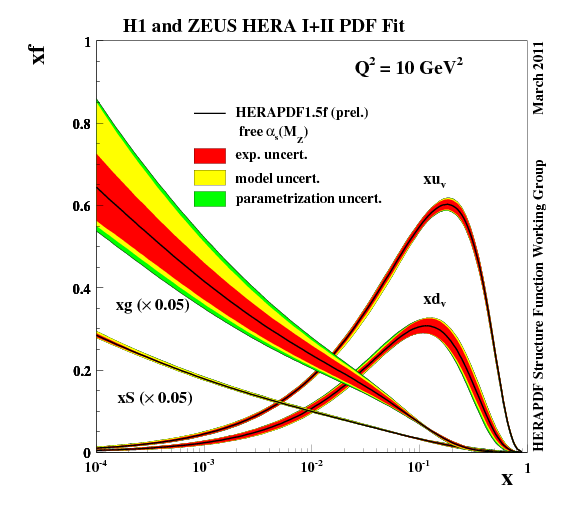
\includegraphics[width=0.8\textwidth]{prevplots/herapdf15f_alpha.png}
  \caption[H1 and ZEUS Parton Distribution Functions]{Combined Parton Distribution Function (PDF) results from HERA experiments \citep{Abramowicz2015} shows probability of finding specific species of particles with fractional momentum, $x_{B}$, inside a proton of squared energy $Q^2 = 10$ GeV$^2$. Carrying the bulk of the momentum are the valence up ($xu_v$) and down ($xu_v$) quarks as expected, however at low $x_{B}$, ``sea quarks'' (quarks created by quantum fluctuations, $xS$) and gluons ($xg$) dominate. The gluon PDF, specifically, dwarfs the rest by over a factor of 20 at low x. (xg and xS, the gluon and sea quark PDFs as plotted here are divided by 20 so they would easily fit on the graph)}
  \label{fig:HERAPDF}
\end{subfigure}
    \rule{35em}{0.5pt}
\begin{subfigure}[p]{0.8\textwidth}
  \centering
    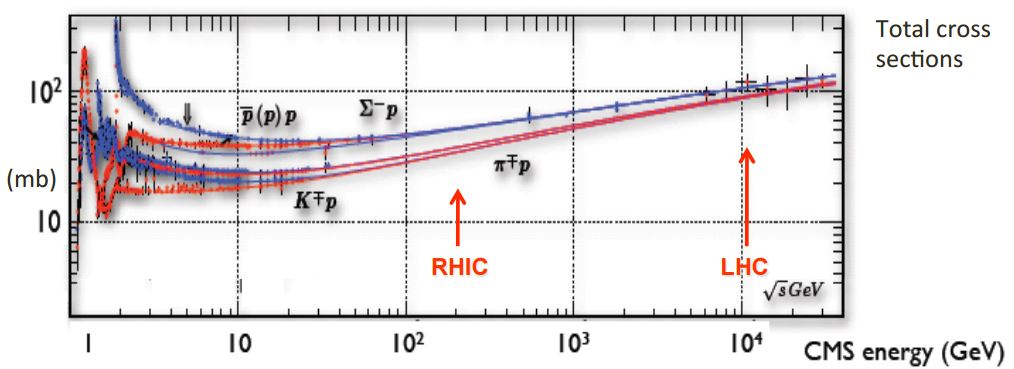
\includegraphics[width=1\textwidth]{prevplots/protoncrosssection.JPG}
  \caption[Proton Cross Section vs Center of Mass Energy.]{Proton Cross Section versus Center of Mass Energy with a variety of probes \citep{PDGcrosssection} \citep{Itakura2012}. Effective cross section increases with energy implying that there is more inside the proton for incident particles to interact with as the energy of the proton increases.}
  \label{fig:PDGxsection}
\end{subfigure}
\end{figure}

\begin{figure}
\centering
\ContinuedFloat
\begin{subfigure}[h]{0.8\textwidth}
  \centering
    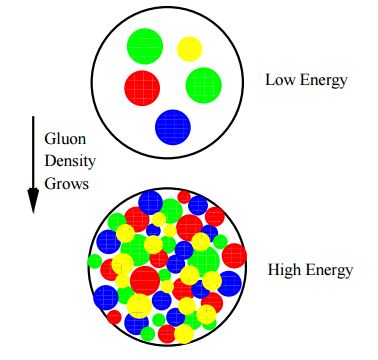
\includegraphics[width=0.5\textwidth]{Figures/gluondensityCGC.jpg}
  \caption[Illustration of gluon saturation in Color-Glass Condensate.]{An illustration of gluon saturation for high energy nucleons \citep{McLerran:2001sr}. As energy increases, the occupation of space by low $x_{B}$ gluons increases.}
  \label{fig:gluonsaturation}
    \rule{35em}{0.5pt}
\end{subfigure}
\caption{}
\end{figure}

Additional support for the model comes from the experimental cross section versus energy. The hadron cross section quantifies the likelihood of a scattering event for an incident beam on a hadron. The classical limit of this cross section is the cross sectional area of a target, but for high energy physics it quantifies the number of interactions that could take place inside of a target (in this case a proton). Figure \ref{fig:PDGxsection} shows that the proton cross section increases above its geometrical cross section ($\pi R_{prot}^2 =$ 30 mb${^-1}$) to over 100 mb$^{-1}$ \citep{PDGcrosssection}\citep{Itakura2012}. That is, as the energy of a proton increases, it fills with ``something'' that can interact with incident particles, resulting in an increase of the interaction cross section above the geometrical cross section. Given the PDF at low \textit{$x_{B}$}, it is extremely likely that this ``something'' is an abundance of gluons.

The increase in the number of gluons in high energy protons has interesting implications in the context of Lorentz contracted nucleons. Longitudinally (i.e., along the direction the proton travels), the valence quarks are flattened together due to this contraction; but transversely, the radius of the proton does not change. This leads to a diminishing amount of space inside the proton for the ever-increasing number of these low \textit{$x_{B}$} gluons to occupy. However, from the PDF, we know that the numbers of gluons have to \textit{increase} as we increase the energy of the proton, and thereby go to lower and lower \textit{$x_{B}$} for constituent gluons. This implies that the lower the fractional momentum, the more \textit{saturated} the proton becomes with gluons, even more so in larger nuclei systems\footnote{Larger by a factor of 10.}. This phenomena of large numbers of bosons occupying the same state is where we get the term \textit{condensate} in CGC.

Furthermore, we know that these gluons are force carriers responsible for holding the constituent valence quarks together; however, due to the PDF, we know that they move orders of magnitude slower than the quarks they are binding together. This inhomogeneity of momentum leads to an inhomogeneity of time scales, due to relativistic time dilation. That is, the constituent quarks' relativistic speeds cause the attached slow moving gluons to move incredibly slowly, appearing to be stationary at time scales the high $x_{B}$ valence quarks experience. This relativistically hindered movement, or \textit{frustration}, has drawn analogs to the condensed matter physics term \textit{glass} which is a classification of materials that have the property of behaving like solids on short time scales and flowing like liquids on long ones. 

But to what end can we continue to add gluons? Current experimental evidence\footnote{HERA PDF results.} appears to say that the gluon density can continue to increase boundlessly, but we know that in order to preserve unitarity\footnote{The integrated PDF must equal the total momentum of the proton \citep{HemmickRHIClecture}.}, it must reach some limit at some point. This process is called gluon \textit{saturation} and it implies that nature has a \textit{maximum gluon density} that, when reached, points to the existence of a CGC \citep{HemmickRHIClecture}. Due to the prevalence of valence quarks in heavy ions, gluon saturation can be achieved at lower accelerator energies than with protons, making heavy ion collisions ideal for studying these phenomena.

\subsection{Glasma}
\begin{figure}
\centering
\begin{subfigure}[h!]{0.8\textwidth}
  \centering
    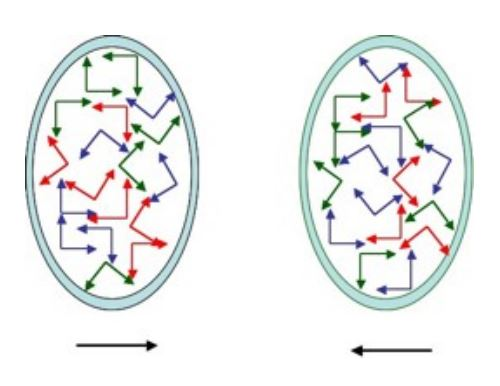
\includegraphics[width=0.4\textwidth]{Figures/collidingCGCsheets.jpg}
  \caption[A cartoon of two color glass sheets just before collision.]{A cartoon of two color glass sheets just before collision. Color fields on the sheets exist only in transverse directions. \citep{McLerran:2008es}} \label{fig:cgcsheets}
\end{subfigure}

\begin{subfigure}[h!]{0.8\textwidth}
  \centering
    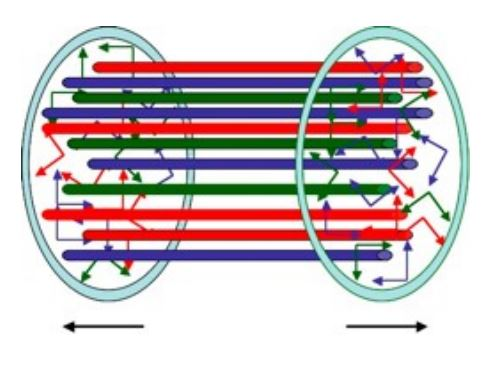
\includegraphics[width=0.4\textwidth]{Figures/glasmatubes.jpg}
  \caption[A cartoon of Glasma formation just after color glass collision.]{A cartoon of Glasma formation. The collision of color glass sheets causes the transverse fields from the two sheets to interact and form cylindrical-shaped, longitudinal fields called \textit{color flux tubes} in the moments just after the collision. \citep{McLerran:2008es}}
 \label{fig:glasmatubes}
\end{subfigure}
    \rule{35em}{0.5pt}
\label{fig:glasmacartoons} \caption{The Formation of Glasma from the collision of Color Glass Sheets.}    
\end{figure}

The CGC has found favor in its ability to describe the initial conditions of the ions before the collision, and relativistic hydrodynamics describes well the thermalized QGP, but the transition from collision to equilibrated phase may be described by another mechanism. This equilibration process, called \textit{thermalization}, can be described by the post-collision behavior of the color fields in the ions \citep{Fujii:2008dd} and depends on the model used to describe the initial conditions. In the moments just before a collision, the ions are Lorentz contracted into a disk-shaped sheet of color glass. The gluon fields on this sheet exist only in the transverse directions as shown in Figure \ref{fig:cgcsheets}. At the moment of impact, the fields interact, and it can be shown \citep{Fries:2006pv} that the resulting color fields of this interaction are all longitudinal and must have a net colorless charge for any transverse cross sectional circle whose radius is $> 1/Q_s$. These fields may possess color charge within this cross sectional circle which projects a cylindrical tube of color charge in space (as shown in Figure \ref{fig:glasmatubes}), sometimes called \textit{Color Flux Tubes}. The overall behavior of this thermalization process through the formation and evolution of color flux tubes is a time dependent, intermediary stage between the CGC and QGP called the \textit{Glasma}, a portmanteau of \underline{\textbf{Glas}}s plas\underline{\textbf{ma}}, so named since it shares properties of both the initial and thermalized states, however it is clearly a new state of matter altogether.

\subsection{Strangeness Enhancement}
The enhancement of strange particle production has historically been promoted as a sign of QGP formation. As mentioned in Section \ref{sect:earlyexperiments}, NA49 and WA97 collaborations observed the enhancement of kaons compared to pions in their measurements. Kaons provide an interesting probe into the mechanisms inside the QGP since they do not exist prior to the collision, rather, they are created freshly from interactions within the newly produced medium. Rafelski and Hagedorn calculated the rates for the production of strange quarks\citep{statmechofquarks} and found that strange quark production was greater than light flavor quark\footnote{Up and down (anti)quarks.} production in the QGP, implying that an increase in strange hadron production could also be a sign of the nuclear phase transition. Furthermore, strange hadrons are easily measured in heavy ion collisions. Berndt M\"ueller noted that, since ``quark flavor is conserved under strong interaction [...], strange quarks, once produced\footnote{By pair processes, $\rightarrow q\bar{q}$.}, are not easy to destroy during the [...] freeze-out stage of a heavy ion reaction.'' \citep{Muller:2011tu} In the context of the CGC model, strange quarks could be plentiful given the abundance of gluons and that $gg \rightarrow s \bar{s}$ is the dominant channel for producing strange quarks \citep{PhysRevLett.48.1066}.

\section{Moving Forward}
I will show that there is sufficient evidence to say that the nuclear matter created by d+Au behaves collectively and that there should be a non-zero elliptic flow measurement. Furthermore, this elliptic flow is dependent on particle species in that it exhibits baryon enhancement in the mid $p_T$ range, indicative of the formation of a QGP. Unknown phenomenon of interest is the enhancement of strangeness. Proton and pion flow is an indicator of first generation quark recombination due to the presence of these quarks in atomic nuclei, however strange quarks do not exist in the nucleus and are rather created ``fresh'' from the QGP.  Evidence of strangeness enhancement via kaon flow independent of quark scaling may be further evidence of QGP formation in the previously thought-to-be-cold d+Au system. Due to system geometry, flow effects should be maximal with the most central collisions since they create the most interaction of nuclear material (see Section \ref{sect:recombcold}). Furthermore, as the collisions become more peripheral, the behavior of the system should become more p+p like.
\pagebreak
\pagebreak
